%--------------------------------------------------------------------
\medskip
\section{Roles Tácticos}
\label{roles}
La implementación de los roles tácticos la hemos realizado a través de la interfaz \texttt{TacticalRole} que contiene dos métodos importantes:
\begin{itemize}
 \item Método \texttt{initialize()}. Este método realiza la inicialización de la estructura táctica que se va a utilizar. Por ejemplo, en el caso de que un rol se implemente con una máquina de estados, pues crear e inicializar dicha máquina.
 \item Método \texttt{update()}. Este método realiza la actualización de la estructura táctica inicializada y las acciones pertinentes dependiendo de dicha actualización.
\end{itemize}

Ambos métodos reciben como parámetro el personaje al que se va a aplicar los comportamientos obtenidos tras la inicialización/actualización de la estructura táctica. \\

También contiene los siguientes métodos:
\begin{itemize}
 \item \texttt{getVelocityFactor()}. Devuelve el factor de velocidad que un rol tiene para un determinado terreno. Este método devolverá un valor entre 0 y 1 que se usa para modificar la velocidad que se aplica a un personaje antes de aplicar un determinado steering. Con este método, se permite que los personajes, dependiendo de su rol, vayan a una velocidad dependiendo del terreno por el que vayan.
 \item \texttt{getTacticalCost()}. Devuelve el coste táctico que un rol tiene asociado a un determinado terreno. 
 \item \texttt{getMaxDistanceOfAttack()}. Devuelve la máxima distancia de ataque de un rol.
 \item \texttt{getDamageToDone()}. Devuelve el daño que puede hacer al atacar un rol.
 \item \texttt{getMaxSpeed()}. Devuelve la máxima velocidad a la que puede ir un rol.
\end{itemize}

Los roles tácticos que hemos implementado nosotros han sido: soldado y arquero, tanto ofensivos como defensivos. Tanto los ofensivos como los defensivos, tienen los mismos valores para los métodos anteriores (dependiendo de si son arqueros o soldados). La diferencia entre ellos está en la estructura con la que se han implementado: los roles ofensivos (tanto soldados como arqueros) se han implementado con un árbol de decisión; mientras que los roles defensivos (tanto soldados como arqueros) se han implementado con una máquina de estados. En las siguientes subsecciones, se comentará más en profundidad sobre cada uno de estos roles. \\

En esta interfaz también podemos encontrar una constante denominada \texttt{health\_cure}. Esta constante indica el ritmo con el que todas las unidades (independientemente del rol concreto) recuperan su vida cuando se están curando. \\

Todo esto se encuentra dentro del paquete \texttt{com.mygdx.iadevproject.aiTactical.roles} del proyecto.


%--------------------------------------------------------------------
\medskip
\subsection{Roles defensivos}
Ambos roles defensivos (arquero y soldado) se han implementado como una máquina de estados. Para ello, se ha hecho uso de la interfaz \texttt{StateMachine} proporcionada por la librería LibGDX \cite{stateMachine}. Esta máquina de estados hace uso de la interfaz \texttt{State} proporcionada también por la librería LibGDX, que proporciona los siguientes métodos:
\begin{itemize}
  \item \texttt{enter()} que se llama cada vez que se entra al estado. 
  \item \texttt{update()} que se llama cada vez que la máquina de estados se actualiza y este es el estado actual de la máquina.
  \item \texttt{exit()} que se llama cuando se sale del estado.
  \item \texttt{onMessage()} que se llama si la entidad recibe un mensaje del despachador de mensajes mientras está en este estado. 
\end{itemize}

Estos métodos reciben como parámetro una entidad con la que se puede trabajar en cada método. En nuestro caso, esta entidad será un objeto de la clase \texttt{Character}. \\

La interfaz \texttt{StateMachine} proporciona varios métodos para poder realizar distintas acciones con la máquina de estados. De entre ellos, las que hemos utilizado son:
\begin{itemize}
 \item \texttt{setInitialState()}. Se emplea para establecer el estado inicial de la máquina, que se le pasa como parámetro.
 \item \texttt{isInState()}. Comprueba si la máquina está en el estado pasado como parámetro.
 \item \texttt{changeState()}. Cambia el estado actual al estado pasado como parámetro.
 \item \texttt{update()}. Actualiza la máquina: esto implica llamar al método \texttt{update()} del estado actual. 
\end{itemize}

Al crear la máquina de estados, esta pide que se indique el objeto ``propietario'' de la máquina de estados; esto es, el objeto que la máquina pasa como parámetro en los métodos de la interfaz \texttt{State}. Para introducirle los estados que nosotros queremos a la máquina de estados, hemos tenido que crear clases concretas que implementaran la interfaz \texttt{State} anteriormente mencionada. Para todos los estados, la entidad que recibe como parámetro es de la clase \texttt{Character}. \\

Por último, en las Figuras \ref{defensivos:soldado} y \ref{defensivos:arquero} se muestran las máquinas de estados concretas para los soldados y arqueros defensivos. La idea que hay detrás de estos roles es que ambos tienen que patrullar una zona (los soldados patrullan su base, los arqueros patrullan los waypoints de los puentes), hasta que se encuentran a un enemigo cerca y lo atacan, siempre y cuando no estén lejos de su base/waypoint. Como se trata de un rol defensivo, estos van a estar atacando hasta que se mueran. Por último, debido a que hay 6 waypoints para cada patrullar, si hay más arqueros defensivos que waypoints, estos se quedarán a la espera (haciendo cosas aleatorias) de que uno se libere para cogerlo. Tanto en el caso del arquero como en el soldado, cuando están yendo hacia un lugar determinado, o en el caso del arquero cuando está a la espera de reservar un waypoint, si se acerca cualquier enemigo o si le atacan, el personaje no hará caso y seguirá haciendo su acción correspondiente. El motivo principal de esta decisión es que al tratarse de roles defensivos, su misión es defender tanto la base como los waypoints de los puentes. Por lo que su prioridad es ir hacia esos puntos y una vez allí atacar a todos los enemigos que se acerquen.
\begin{figure}[!th]
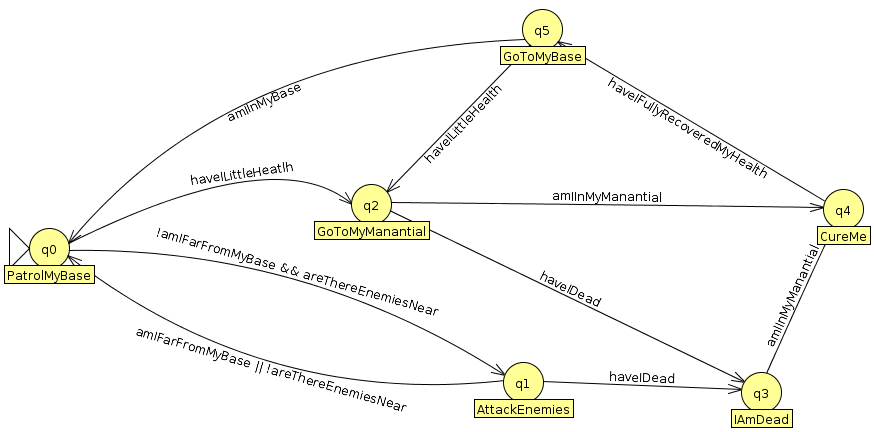
\includegraphics[scale=0.6]{defensive-soldier}
\centering
\caption{Máquina de estados para el soldado defensivo.}
\label{defensivos:soldado}
\end{figure}
\begin{figure}[!th]
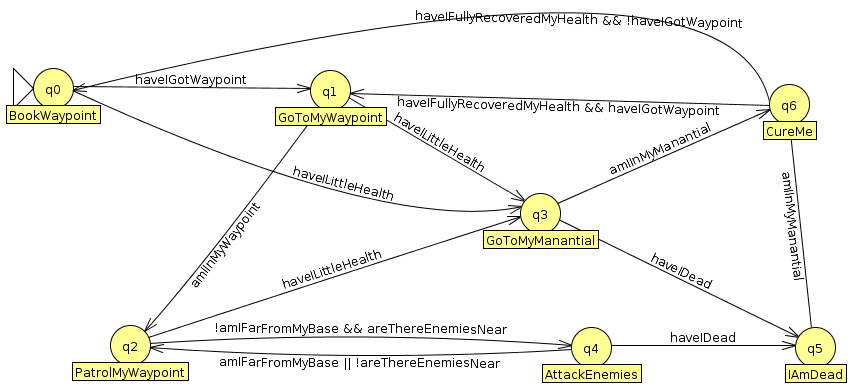
\includegraphics[scale=0.6]{defensive-archer}
\centering
\caption{Máquina de estados para el arquero defensivo.}
\label{defensivos:arquero}
\end{figure}

\newpage
Es importante destacar los siguientes puntos:
\begin{itemize}
 \item Si no se cumplen las condiciones necesarias en el estado actual, no se cambia de estado. De ahí que no haya transiciones en las figuras sobre los propios estados. Cuando no se cambia de estado, exceptuando el estado \texttt{AttackEnemies} y los que requieren el uso del Pathfinding, la máquina de estados no se actualiza, ya que cuando se entró al estado, se calcularon los comportamientos correspondientes y el personaje sigue haciendo lo mismo, por lo que no es necesario calcularlo de nuevo.
 
 \item Los estados que requieran el uso del Pathfinding (\texttt{GoToMyBase, GoToMyManantial y GoToMyWaypoint}) para evitar que se esté calculando el Pathfinding cada vez que se actualice el estado, hacemos uso del método \texttt{enter()} del estado para que cada vez que se entre se calcule el Pathfinding, mientras que en el método \texttt{update()} lo que se hace es aplicar el Pathfinding para que nos dé el siguiente punto a seguir.
 
 \item En el estado \texttt{AttackEnemies} se ataca siempre al enemigo más cercano (de ahí que se tenga que actualizar el estado si no hemos cambiado). También el personaje intenta alejarse del objetivo a una distancia en la que él pueda atacar. Así pues permitimos que aquellos personajes que tengan una distancia de ataque mayor (los arqueros en nuestro caso), puedan sacar provecho de ello cuando se ataca. También se mira al personaje que se ataca.
 
 \item En el estado \texttt{IAmDead} se traslada directamente el personaje a la posición de su manantial, estableciendo su posición a la posición del manantial.
 
 \item En el estado \texttt{BookWaypoint} mientras que espera a tener un waypoint libre, el personaje lo que hace es moverse de manera aleatoria (aplicando un Wander), para evitar que se quede parado.
 
 \item Debido a que los arqueros defensivos tienen que reservar el waypoint que tienen que patrullar, solamente se va a liberar un waypoint cuando el arquero que lo está patrullando muere. Es decir, entrar al estado \texttt{IAmDead} implica que el arquero deja libre su waypoint para que otro pueda cogerlo. Sin embargo, cuando un arquero entra al estado \texttt{GoToMyManantial} porque quiere curarse, no se libera el waypoint porque no ha muerto. 
 
 \item Los estados de patrulla \texttt{PatrolMyBase y PatrolMyWaypoint}, en ambos casos, consiste en realizar un seguimiento de los waypoints establecidos. En el caso de las bases son waypoints alrededor de la base, mientras que en el caso de los puentes, un arquero patrulla el waypoint que tiene reservado y su vecino.
 
 \item Consideramos que de primeras, los soldados se encuentran en la base (o cerca de ella), por lo que en su estado inicial no se hace ningún Pathfinding. En cambio, como los arqueros, mientras que no tienen un waypoint que patrullar, se mueven de manera aleatoria, cuando reserva un waypoint, sí se calcula un Pathfinding para ir a él, porque pueden estar en la otra punta del mapa.
\end{itemize}


%--------------------------------------------------------------------
\medskip
\subsection{Roles ofensivos}
Tanto el arquero ofensivo como el soldado ofensivo han sido implementados con \textbf{árboles de decisión}. Los correspondientes arboles se puede encontrar en las propias clases \texttt{OffensiveSoldier} y \texttt{OffensiveArcher}. En estas clases podemos observar una serie de atributos que representan cada uno de los nodos hoja a los que el árbol de decisión podrá llegar (en cada nodo hoja se realizarán una serie de acciones). Además de los nodos hojas, también podemos encontrar otro atributo llamado \texttt{lastNode}. Aunque estemos tratando con un árbol de decisión y aunque cada vez que lo llamemos se realicen todos las comprobaciones (desde el principio hasta que una se cumpla), es bastante necesario contar con un mecanismo para \textit{recordar} cual es el último nodo hoja al que llegamos. Esto es necesario, debido a que al llegar a un nodo hoja a través de las ramas del árbol, en algunos casos será necesario realizar ciertas acciones sobre el nodo anterior en el que nos encontrábamos (protocolo de salida del nodo anterior). Esto solamente se hará en caso de que el último nodo hoja y el actual al que hemos llegado sean distintos. \\

Además de los atributos mencionados, en las clases \texttt{OffensiveSoldier} y \texttt{OffensiveArcher} hay un método llamado \texttt{update}. Tal y como se ha comentado antes, este método realiza la actualización de la estructura táctica. Para el caso concreto de los árboles de decisión, el método \texttt{update} empezará a ```recorrer el árbol'' (en profundidad y de izquierda a derecha) hasta que las condiciones pertinentes (checks) se cumplan y podamos llegar a un nodo hoja (esto se ha implementado con sentencias \textit{if-else}). \\

Una cosa importante a tener en cuenta es que al llegar a un nodo hoja del árbol, antes de ejecutar dicho nodo hoja deberemos comprobar si el nodo al que hemos llegado es distinto de \texttt{lastNode} (nodo anterior al que se llegó). En caso afirmativo, se ejecutará el \textbf{método de salida del nodo anterior}, a continuación, el \textbf{método de entrada} del nuevo nodo hoja al que hemos llegado y, finalmente, ya podremos proceder a la ejecución de dicho nodo hoja (el nuevo nodo hoja se asigna a \texttt{lastNode}). Otra cosa importante a tener en cuenta es que los árboles de decisión no requieren inicialización (el método \texttt{initialize} está vacío). \\

Puesto que la finalidad de todo personaje ofensivo es ir a atacar al enemigo a su base (a la base del enemigo) y, también, atacar a todo enemigo que se le ponga por delante, el árbol de decisión de los soldados ofensivos será el mismo que el de los arqueros ofensivos. Las nodos hojas a los que podemos llegar son los siguientes:
\begin{itemize}
	\item \texttt{IAmDead} $\rightarrow$ Cuando la vida de un personaje llega a 0, éste es trasladado directamente a la posición de su manantial, estableciendo su posición a la posición del manantial. Este nodo no requiere método de entrada ni método de salida. Puesto que en un árbol siempre se ejecutan todas las comprobaciones hasta llegar a un nodo hoja y debido a que este nodo está el primero, cuando movamos el personaje a la fuente, \textbf{debemos poner a uno su vida}. Si no hacemos esto, el árbol de decisión se quedará pillado en esta comprobación (porque al tener vida 0, siempre se considerará que estoy muerto) y el personaje no funcionará correctamente (jamás podremos pasar de la primera rama del árbol).
	\item \texttt{GoToMyManantial} $\rightarrow$ En este nodo le decimos al personaje que tiene ir a curarse a su manantial. Puesto que esto requiere un pathfinding (que será un atributo del nodo), este estado sí tiene un método de entrada. Este método de entrada crea el objeto pathfinding y lo almacena en el propio nodo.
	\item \texttt{CureMe} $\rightarrow$ En este nodo debemos decirle al personaje (ya en el manantial) que debe regenerar su nivel de vida. Además, mientras que ese nivel de vida no llegue al máximo, el personaje deberá permanecer en el manantial (aplicando un comportamiento que constantemente lo lleve a la posición del manantial). Para el caso de las formaciones, los mecanismos de ataque y cura se han implementado de una manera diferente al resto de personajes normales (se comentará en el apartado correspondiente), por ese motivo, este nodo va a necesitar un método de salida para indicar este hecho (que los componentes de la formación deben parar de curarse).
	\item \texttt{GoToEnemyBase} $\rightarrow$ En este nodo se indica al personaje que debe ir a la base enemiga. Al igual que pasaba la acción de ir al manantial, este nodo requerirá un pathfinding y, por tanto, un método de entrada.
	\item \texttt{AttackEnemies} $\rightarrow$ En este nodo se indica al personaje (de manera apropiada, según sea un personaje normal o una formación) que debe atacar a un determinado objetivo (el enemigo más cercano). Para poder llevar a cabo ese ataque, el personaje se posicionará en la posición adecuada según la distancia desde la que pueda atacar (depende de si es un arquero o un soldado). Al igual que pasa con la cura de los personajes, las formaciones se tratan de una forma distinta y, por tanto, este nodo va a necesitar un método de salida (para indicar a los componentes de la formación que deben parar de atacar).
	\item \texttt{Win} $\rightarrow$ En este nodo, el equipo al que pertenece el personaje ha ganado. Las condiciones de victoria y como se han gestionado estos elementos se explicará en el apartado correspondiente.
\end{itemize}

Para generalizar y trabajar de manera homogénea con todos los nodos hoja, se ha creado la interfaz \texttt{Node}. Todos los nodos la implementarán. \\

Hay que tener muy claro que, debido a que en un árbol de decisión siempre se hacen todas las comprobaciones posibles desde el principio hasta llegar a un nodo hoja, hay que tener mucho cuidado en el diseño del árbol y en qué ramas se ponen antes que otra. Si no hacemos esto, podremos llegar a situaciones raras que podrán provocar efectos no deseados sobre el comportamiento táctico del personaje. En la Figura \ref{ofensivos:ofensivos} se puede observar una representación del árbol de decisión (que, como se ha comentado antes, es el mismo para los arqueros y soldados ofensivos). \\

\begin{figure}[!th]
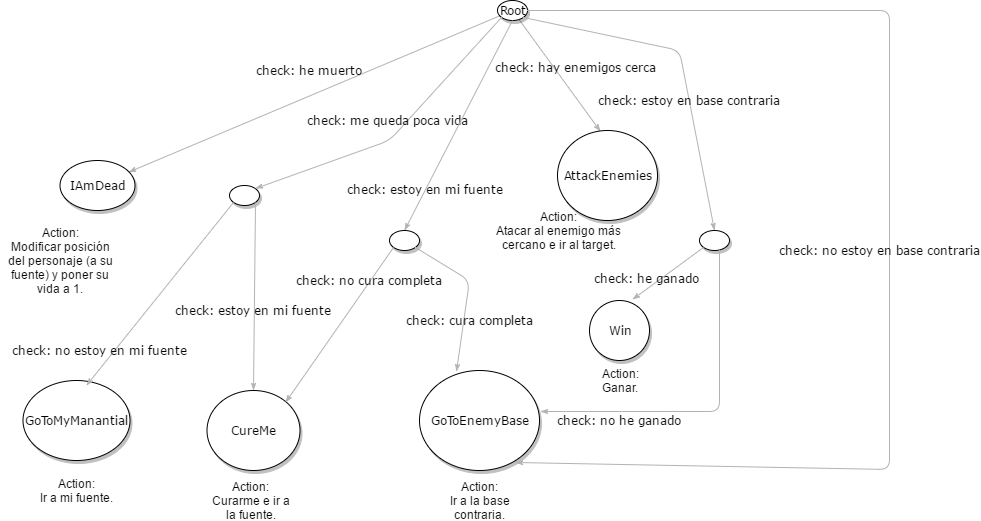
\includegraphics[scale=0.5]{arbolDecisionOfensivo}
\centering
\caption{Árbol de decisión para los arqueros y soldados ofensivos.}
\label{ofensivos:ofensivos}
\end{figure}

Tal y como se puede observar, todo aquello que necesite un pathfinding estará lo más a la derecha posible en el árbol.
